\documentclass[a4paper,10pt]{article}
\usepackage{geometry}[2cm,2cm,2cm,2cm]
\usepackage[utf8]{inputenc}
\usepackage{amsmath,amsfonts,amssymb,amsopn}
\usepackage[colorlinks]{hyperref}
\usepackage{color}
\usepackage{graphicx}



%opening
\title{Fully implicit timestepping methods for the rotating shallow water equations}
\author{Werner Bauer\footnote{University of Surrey, UK (w.bauer@surrey.ac.uk), Ochid: ???} \ and
Colin J. Cotter\footnote{Imperial College London, UK, Orchid: ???}  }


\newcommand{\todo}[1]{\vspace{5 mm}\par \noindent
	\framebox{\begin{minipage}[c]{0.95 \textwidth}
			\tt #1 \end{minipage}}\vspace{5 mm}\par}
\newcommand{\checkit}[1]{{\color{red}#1}}
\newcommand{\werner}[1]{{\color{magenta}WB says: #1}}
\newcommand{\incl}[1]{{\color{red}#1}}



\DeclareMathOperator{\sat}{sat}
\newcommand{\DD}[2]{\frac{D #1}{D #2}}
\newcommand{\V}{\mathbf{V}}
\newcommand{\U}{\mathbf{U}}
\newcommand{\W}{\mathbf{W}}
\newcommand{\M}{\mathrm{M}}
\newcommand{\R}{\mathrm{R}}
\newcommand{\La}{\mathrm{L}}
\newcommand{\Fu}{\mathbf{F}}


% \newcommand{\D}{\mathbf{D}}
\newcommand{\N}{\mathbf{N}}
\newcommand{\tN}{\tilde{N}}
\newcommand{\tk}{\tilde{k}}
\newcommand{\opL}{\mathcal{L}}
\newcommand{\opN}{\mathcal{N}}



\def\MM#1{\boldsymbol{#1}}
\newcommand{\pp}[2]{\frac{\partial #1}{\partial #2}}
%\newcommand{\dede}[2]{\frac{\delta #1}{\delta #2}}
\newcommand{\dd}[2]{\frac{\diff#1}{\diff#2}}
\newcommand{\dt}[1]{\diff\!#1}
\def\MM#1{\boldsymbol{#1}}
\DeclareMathOperator{\diff}{d}
\DeclareMathOperator{\Tr}{Tr}
\DeclareMathOperator{\uu}{\MM{u}^\delta}
\DeclareMathOperator{\F}{\MM{F}^\delta}
\DeclareMathOperator{\D}{D^\delta}
\DeclareMathOperator{\q}{q^\delta}
\DeclareMathOperator{\Z}{Z^\delta}
\DeclareMathOperator{\qr}{\mathring{q}^\delta}
\DeclareMathOperator{\DIV}{DIV}




\begin{document}

\maketitle

\begin{abstract}
Fully implicit timestepping methods have several potential advantages for atmosphere/ocean simulation. First, being unconditionally stable, they degrade more gracefully as the Courant number increases, typically requiring more solver iterations rather than suddenly blowing up. Second, particular choices of implicit timestepping methods can extend energy conservation properties of spatial discretisations to the fully discrete method. Third, these methods avoid issues related to splitting errors that can occur in some situations, and avoid the complexities of splitting methods.

Fully implicit timestepping methods have had limited application in geophysical fluid dynamics due to challenges of finding suitable iterative solvers, since the coupled treatment of advection prevents the standard elimination techniques. However, overlapping Additive Schwarz methods, as introduced for geophysical fluid dynamics by Cotter and Shipton (2023), provide a robust, scalable iterative approach for solving the monolithic coupled system for all fields and Runge-Kutta stages.

In this study we investigate this approach applied to the rotating shallow water equations, facilitated by the Irksome package (Farrell et al, 2021) which provides automated code generation for implicit Runge-Kutta methods. We compare various schemes in terms of accuracy and efficiency using an implicit/explicit splitting method, namely the ARK2 scheme of Giraldo et al (2013), as a benchmark. This provides an initial look at whether implicit Runge Kutta methods can be viable for atmosphere and ocean simulation.
\end{abstract}

\section{Introduction}


\section{Fully implicit Runga Kutta methods and monolithic solver strategy}

We develop a method suitable to solve fully implicit Runga-Kutta methods, implicit over all stages of the RK methods. First, we recall RK methods, especially those that are fully implicit and that can be formulated with the Irksome library. This gives fully implicit systems that need a careful solver selection in order to be efficiently solved.


\subsection{Fully implicity Runga Kutta (RK) time integration methods}

We consider the ODE $y'(t) + F(t,y)= 0$ where $y:(0,T] \rightarrow \mathbb{R}^n$ with $y(0) = y_0$
and $F:(0,T]\times \mathbb{R}^n \rightarrow \mathbb{R}^n$.
Given the solution
$y(t^n)\equiv y^n$ and some $t^{n+1} = t^n + \Delta t$, Runga-Kutta (RK) methods approximate $y(t^{n+1})$ by
$y^{n+1} = y^{n} + \Delta t \sum_{i = 1}^{s} b_i k_i,$ where for all $1\leq i \leq s$
 the stages $k_i \in \mathbb{R}^n$ satisfy
\begin{align*}
%  y^{n+1} = y^{n} + \Delta t \sum_{i = 1}^{s} b_i k_i, \
%  \text{where for all $1\leq i \leq n$
%  the stages $k_i \in \mathbb{R}^n$ satisfy} \\
 k_i + F\Big(t + c_i \Delta t, \  y + \Delta t \sum_{j = 1}^{s} A_{ij} k_j \Big) = 0 \
 \text{with $A_{ij}, b_i, c_i$ for $1\leq i,j\leq s$.}
\end{align*}
$A_{ij}, b_i, c_i$ are typically organized in a \emph{Butcher tableau} and determine the order of accuracy.


\subsection{Solver strategy of fully implicit monolithic systems}

\noindent \textcolor{blue}{\textbf{Monolithic solver}}

  Such solver treats the full system of coupled variables (over all stages)
  without elimination. To solve the nonlinear algebraic system from an
  implicit RK method we use:
  \begin{itemize}
  \item Nonlinear system solver: \emph{linesearch Newton},
  \item Jacobian solver (for $J$ evaluated at current Newton state):
    \emph{Preconditioned GMRES},
  \item Preconditioner: \emph{monolithic geometric multigrid (V cycle)},
  \item Multigrid smoothers: \emph{additive Schwarz method (ASM)}.
  \end{itemize}

\vspace{0.7cm}

\noindent \textcolor{blue}{\textbf{Additive Schwarz method (ASM)}}

The mesh is decomposed
  into overlapping patches, and the fully coupled Jacobian is solved
  independently (and hence parallelisably) on each patch. The result
  of the smoother is the sum of the solutions over all of the
  patches. In this work, a ``vertex star'' patch is used: it includes
  all of the degrees of freedom in the cells sharing one vertex,
  excluding those associated to the boundary (see Figure 1). For
  3D/vertical slice models, column patches are formed from all the
  cells sharing a vertex star patch on the horizontal base mesh (see
  Cotter and Shipton (2023)).


\vspace{0.7cm}


\noindent \textcolor{blue}{\textbf{Solver performance: linearisation about current state}}

  For the rotating shallow water equations on the sphere linearised
  about a state of rest, the monolithic solver converges at a rate
  that is robust to mesh refinement and changes in $\Delta t$. Figure
  1 shows the average GMRES iterations per timestep to achieve a
  residual reduction of $10^{-10}$, using the ``Williamson 5
  mountain'' initial conditions and topography, run for 1 day. A
  compatible finite element discretisation with BDM2-DG1 spaces on
  triangles is used (3 pressure DOFs and 7.5 velocity DOFs per cell), with Crank-Nicholson
  implicit timestepping.



  \vspace{-5mm}
  \begin{center}
  \parbox{6.2cm}{
    \vspace{1cm}
  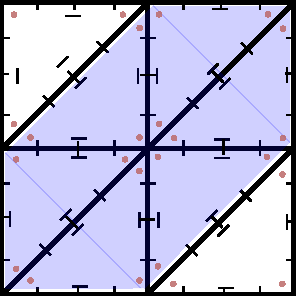
\includegraphics[width=4cm]{Images/patch}}
  \begin{tabular}{ccc}
    Cells & $\Delta t$ & its/step \\
    \hline
    20480 & 3600s & 8 \\
    81920 & 3600s & 8 \\
    327680 & 3600s & 8 \\
    20480 & 1800s & 8 \\
    20480 & 7200s & 8 \\
    20480 & 14400s & 8.6 \\
  \end{tabular} \\
  \vspace{2mm}
  {\bfseries Figure 1}: (LEFT) a diagram showing the ``vertex star'' patch. (RIGHT)
  iteration counts for the monolithic solver applied to the linear
  rotating shallow water equations on the sphere.
  \end{center}



 \noindent \textcolor{blue}{\textbf{Solver performance: Nonlinear rotating shallow water equations}}

 For the nonlinear rotating shallow water equations, the introduction
 of advection terms degrades $\Delta t$ robustness but mesh independent
 iteration counts are achieved upon maintaining a constant Courant
 number (see Figure 2). BDM2-DG1 spaces on triangles are used
 with Crank-Nicholson implicit timestepping.

\begin{figure}[h]
 \begin{tabular}{cccc}
    Cells & $\Delta t$ & GMRES its/step & Wallclock \\
    \hline
    20480 & 3600s & 18.86 & 16m45s \\
    81920 & 1800s & 18.03 & 1h26m38s \\
    327680 & 900s & 18.00 & 9h54m50s \\
  \end{tabular}
   \caption{Average number of GMRES
      iterations per timestep, and wallclock times, for nonlinear
      rotating shallow water equations running the ``Williamson 5
      mountain'' testcase until 15 days at various resolutions and
      fixed $\Delta x/\Delta t$ ratio, on 16 cores.}
\end{figure}




\section{Numerical results}


As an example, we applied the monolithic solver approach
to the nonlinear shallow water equation on the sphere.
The equations take the form
 \begin{align*}
   \DD{u}{t} + fk\times u + g \nabla (\rho+b)    & = 0, \\
   \pp{\rho}{t} + \nabla\cdot(u\rho) & = 0,
 \end{align*}
where $u$ is the (horizontal) velocity, $f$ is the Coriolis parameter,
$k$ is the local up direction, $\rho$ is the layer depth, $b$ is the
bottom topography, and $g$ is gravitational acceleration.


\noindent \textcolor{blue}{\textbf{Test case}}
We use Williamson's testcase 6 and run it for 1 day on mesh level 5.
We compare the solutions obtained from the studied time integrators with
large time step size ($dt >18.5s$) with a reference solutions determined with $dt=1s$.
We also record the total runtime of each of these simulations.
Note that the total runtimes depend on the number of CPU-cores!
\vspace{0.6cm}

% \begin{minipage}{0.43\linewidth}\centering
 \begin{figure}[t]\centering
 \begin{tabular}{cc}
 \hspace{-0em}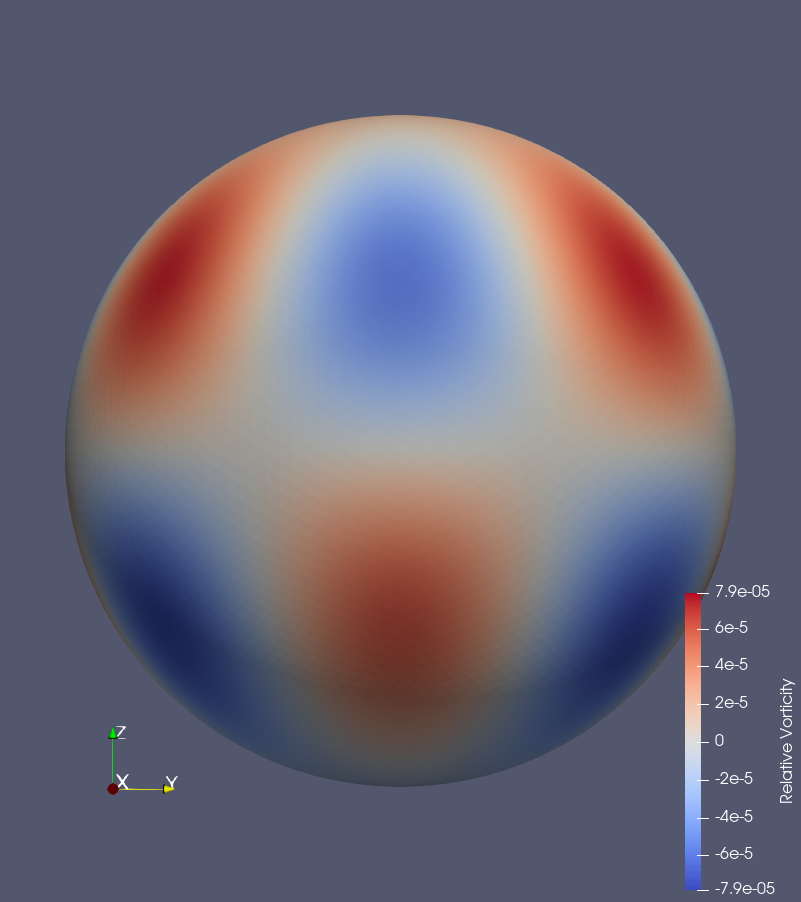
\includegraphics[scale=0.125]{Images/vorticity_0.png} &
 \hspace{-0em}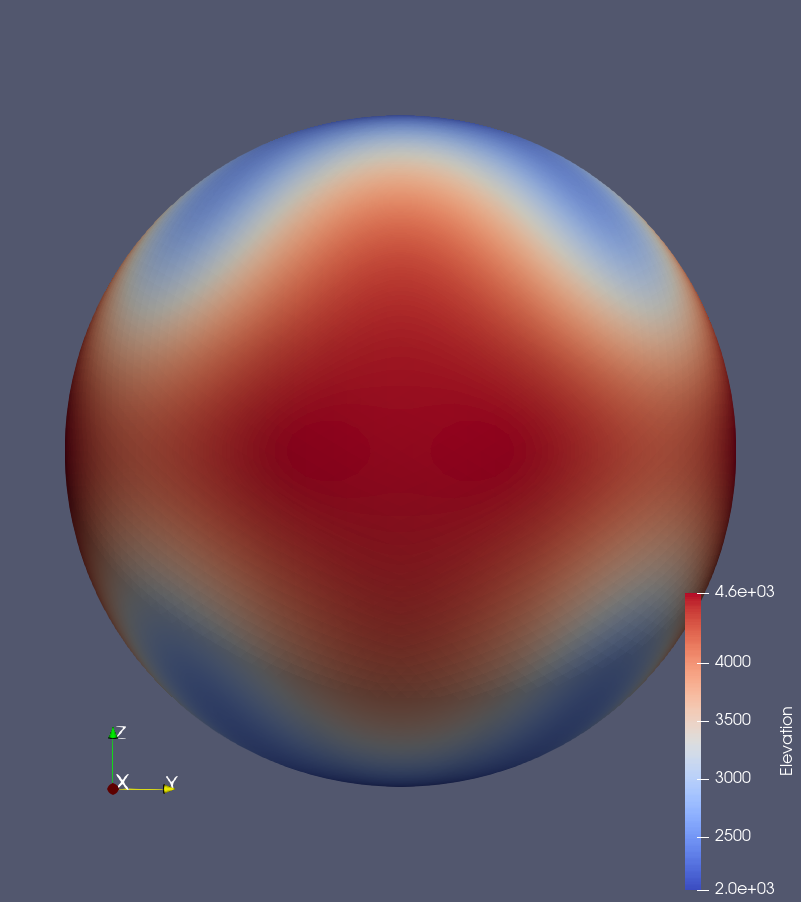
\includegraphics[scale=0.125]{Images/elevation_0.png} \\
 \hspace{-0em}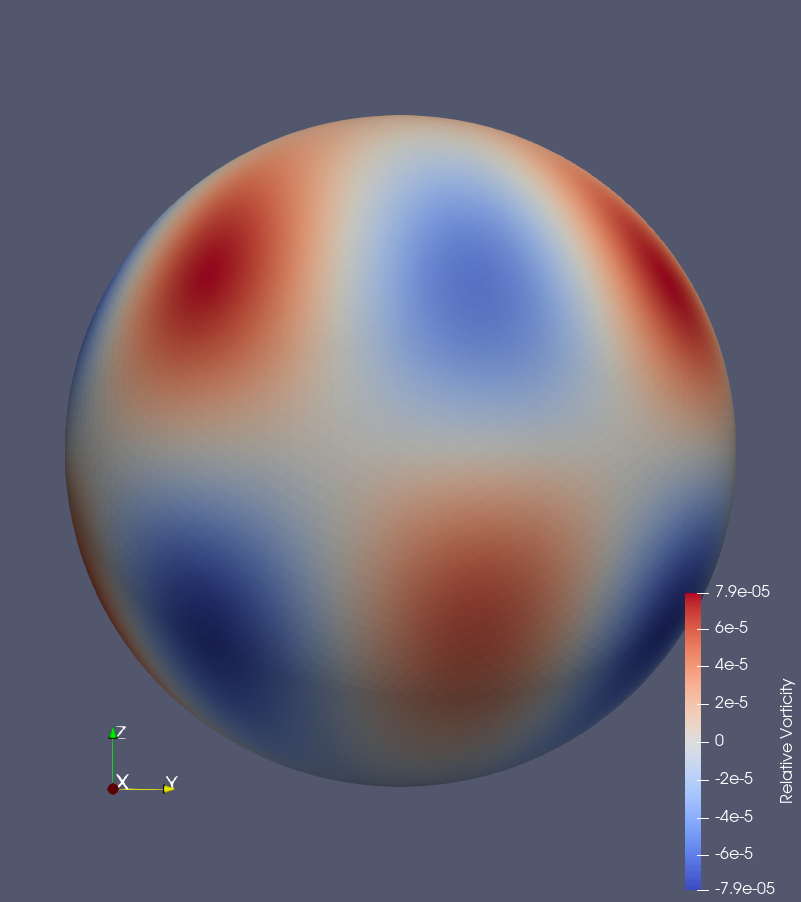
\includegraphics[scale=0.125]{Images/vorticity_24.png} &
 \hspace{-0em}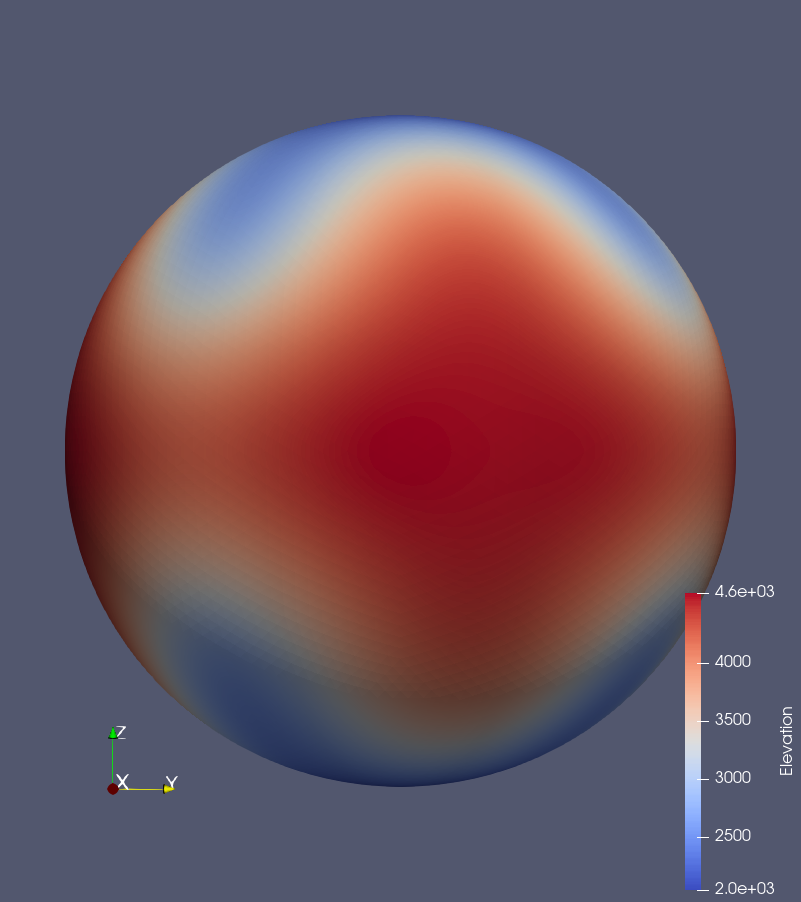
\includegraphics[scale=0.125]{Images/elevation_24.png} \\
 \end{tabular}\vspace{-10pt}
  \caption*{{\bfseries Figure 3}: TOP: initial vorticity (left) and depth (right) fields
  for Williamson test case 6. BOTTOM: fields at day 1. The shown fields are for mesh level 5.
  }
  %\label{fig1}
  \end{figure}
%  \end{minipage}\hfill
% \begin{minipage}{0.55\linewidth}
\begin{figure}[t]\centering
\begin{tabular}{c}
 \hspace{-0.4em}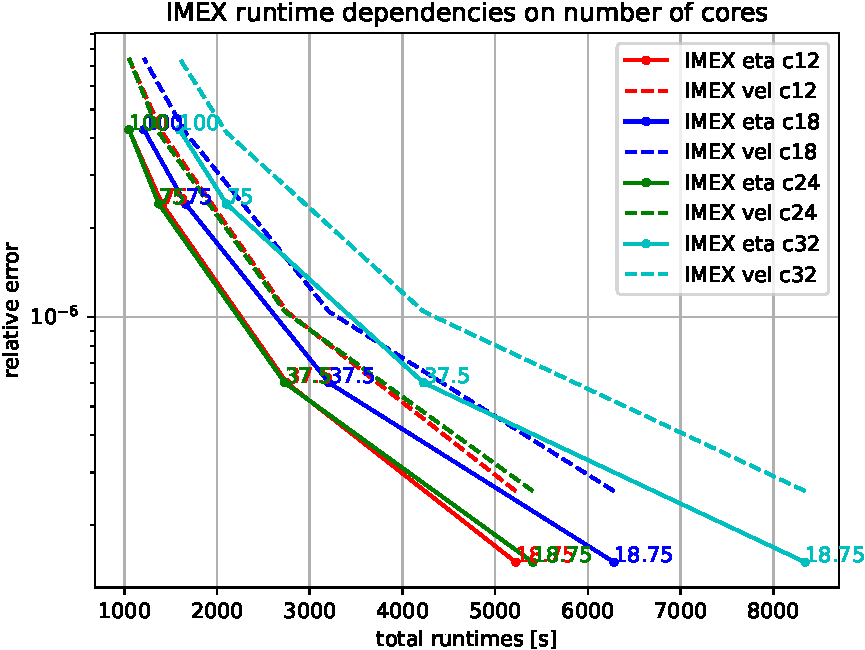
\includegraphics[scale=0.66]{Images/Figure_1_new1-crop.pdf}
  \end{tabular}
\caption*{{\bfseries Figure 4}: dependency of total runtimes
    of IMEX scheme on the number of available CPU-cores.
  }
  %\label{fig1}
  \end{figure}
  \vspace{2cm}
 % \end{minipage}


\noindent \textcolor{blue}{\textbf{Total runtimes vs. relative errors}}

  Figure 5 summarized the numerical results, i.e. total runtimes vs
  relative errors of depth $\rho$ and velocity $ u$ fields for ARK2 IMEX
  scheme, and for Gauss-Legendre (GL) schemes of order 1 (GL1), order 3 (GL2) and order 5 (GL3).

 \begin{figure}[t]\centering
 \begin{tabular}{cc}
 \hspace{-0.2em}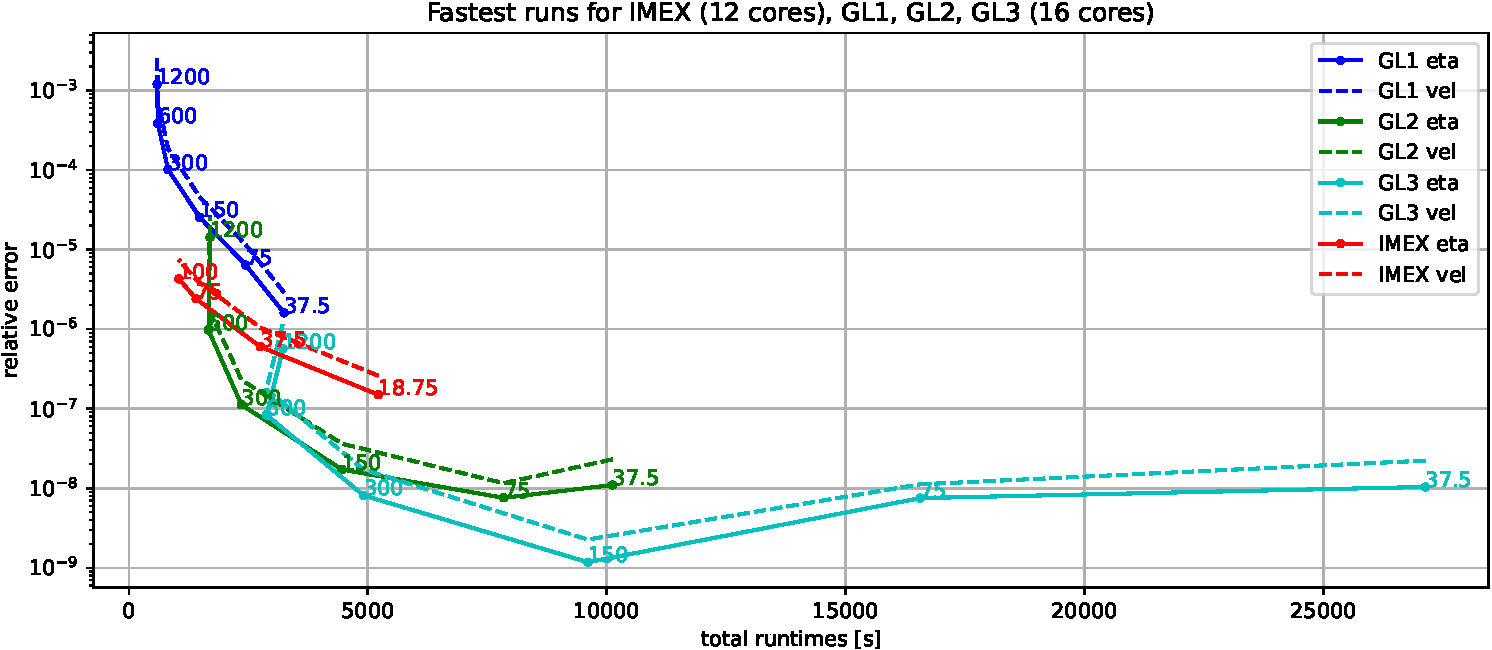
\includegraphics[scale=0.52]{Images/Figure_2_new3-crop.pdf} &
 %\hspace{-0.95em}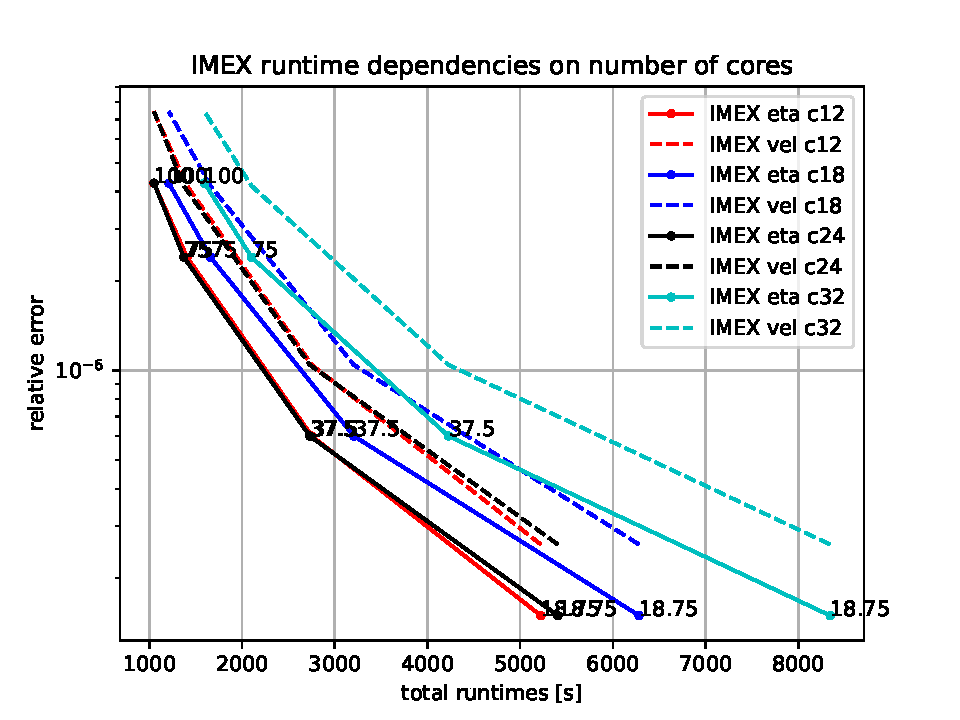
\includegraphics[scale=1.19]{Images/Figure_1_new.pdf}
  \end{tabular}\vspace{-10pt}
  \caption*{{\bfseries Figure 5}: relative errors (y-axis)
  of depth (eta) and velocity (vel) fields against the
  total runtimes of the simulations depending on the chosen schemes
  (IMEX, GL1, GL2, GL3). The total runtimes depend on the schemes,
  the time step sizes (colored figures) and on the number of available CPU-cores
  (cf. Figure 4).

  }
  \label{fig2}
  \end{figure}





 \cleardoublepage


\section{Conclusions}

   \begin{itemize}
    \item Our benchmark tests are \textbf{fair comparisons} between implicit RK schemes (of different orders) from Irksome with the ARK2 IMEX scheme, all using the same monolithic solver in Firedrake.

%    \item Figure 4 shows that under such 'fair' conditions, 3rd-order GL2 is more efficient than 2nd-order ARK2 IMEX: either it is two orders of magnitude more accurate or it requires much less runtime.
   \item Figure 5 shows that under such 'fair' conditions:\\
   (i) 3rd-order GL2 is a little slower than 2nd-order ARK2 IMEX, but about one order of magnitude more accurate; \\
   (ii) 1st order GL1 is slightly quicker but less accurate.

  \item So far, we did not explore advanced solver options, so further speedup for RK methods can be achieved.


   \item Hence, the assumption that IMEX schemes are the fastest schemes for atmosphere/ocean simulation is not necessarily correct.

   \item \textbf{Outlook:} the flexibility of Irksome in easily choosing different accuracy-orders for a vast variety of implicit RK methods allows us to further explore even more efficient time integrators.
   \end{itemize}



\begin{thebibliography}{8}
\bibitem{CotterShipton12} Cotter, Colin J., Jemma Shipton. "Mixed finite elements for numerical weather prediction." Journal of Computational Physics 231, no. 21 (2012): 7076-7091.

\bibitem{CotterShipton23}
\checkit{ADD PAPER DETAILS}

\bibitem{Farrell21} Farrell, Patrick E., Robert C. Kirby, Jorge Marchena-Menendez. "Irksome: Automating Runge-Kutta time-stepping for FE methods." ACM Transactions on Math. Software (TOMS) 47, no. 4 (2021): 1-26.

\bibitem{Giraldo13} Giraldo, Francis X., James F. Kelly, and Emil M. Constantinescu. "Implicit-explicit formulations of a three-dimensional nonhydrostatic unified model of the atmosphere (NUMA)." SIAM Journal on Scientific Computing 35, no. 5 (2013): B1162-B1194.
\end{thebibliography}






\end{document}
